\documentclass[letterpaper, 10 pt, conference]{ieeeconf}  % Comment this 
%\documentclass{article}
%\usepackage{nips10submit_e}
%\documentclass[a4paper, 10pt, conference]{ieeeconf}      % Use this line for a4 paper

%\IEEEoverridecommandlockouts                              % This command is only needed if 
                                                          % you want to use the \thanks command

%\overrideIEEEmargins                                      % Needed to meet printer requirements.

% See the \addtolength command later in the file to balance the column lengths
% on the last page of the document

% The following packages can be found on http:\\www.ctan.org
\usepackage{graphics} % for pdf, bitmapped graphics files
\usepackage{epsfig} % for postscript graphics files
\usepackage{graphicx}
\usepackage{mathptmx} % assumes new font selection scheme installed
\usepackage{times} % assumes new font selection scheme installed
\usepackage{mathtools} % assumes amsmath package installed
\usepackage{amssymb}  % assumes amsmath package installed
\usepackage{tikz}
\usepackage{tabulary}
\newcommand{\hvec}{\overset{\rightharpoonup}}
\newcommand{\argmin}{\arg\!\min}
\newcommand{\norm}[1]{\left\lVert#1\right\rVert}
\newcommand{\quotes}[1]{``#1''}
\usetikzlibrary{calc,positioning, fit, arrows}
%\usepackage{biber}

%for citing webcites
\usepackage{cite}
\usepackage{url}

\makeatletter
\newenvironment{tablehere}
  {\def\@captype{table}}
  {}

\newenvironment{figurehere}
  {\def\@captype{figure}}
  {}
\makeatother

\newcommand{\vect}[1]{\ensuremath{\mathbf{#1}}}
\newcommand{\mat}[1]{\ensuremath{\mathbf{#1}}}
\newcommand{\transpose}{\ensuremath{\mathsf{T}}}
\newcommand{\of}[1]{\ensuremath{\left(#1\right)}}

\title{\LARGE \bf
Lightweight Vision Based Multiple Target Tracking Using Deep Learning and Recursive RANSAC
}


\author{Dallin Briggs}


\begin{document}



\maketitle
\thispagestyle{empty}
\pagestyle{empty}


%%%%%%%%%%%%%%%%%%%%%%%%%%%%%%%%%%%%%%%%%%%%%%%%%%%%%%%%%%%%%%%%%%%%%%%%%%%%%%%%
\begin{abstract}

This report describes the methods used to improve the capabilities of Unmanned Aerial Vehicles in tracking targets autonomously on a lightweight, small platform that requires little computational resources. Unmanned aircraft are becoming increasingly more capable and smaller and the goal of this report is to show that a neural network can be effective in robustly tracking ground targets with small embedded single board computers on-board a small unmanned aircraft. This approach will be leveraging existing work done in this field (Recursive RANSAC) as the primary target tracker and neural networks to learn and classify targets. The target classification will be used in associating targets that are observed multiple times with previous tracks recorded by Recursive RANSAC.

\end{abstract}


%%%%%%%%%%%%%%%%%%%%%%%%%%%%%%%%%%%%%%%%%%%%%%%%%%%%%%%%%%%%%%%%%%%%%%%%%%%%%%%%
\section{INTRODUCTION}

Multiple object tracking (MOT) is currently a popular topic in the deep learning community. It can be used for a variety of cases, but most are typically related to the robotics industry. Unmanned Aerial Vehicles (UAV's) have advanced rapidly in the past decade and are now being used for both military and commercial purposes. A common use case for UAV's in the military is for intelligence, surveillance, and reconnaissance (ISR) missions. 

Currently, military UAV's are usually equipped with expensive gimbaled cameras that are able to view targets such as people or vehicles from a high altitude. Those targets are being tracked by pilots who are remotely controlling the aircraft. This task can be difficult and time consuming for humans to track a target over the course of several hours. In order to improve the capabilities of UAV's to track ground targets autonomously, a neural network is proposed to learn targets and track them even after loosing visual line of sight temporarily.

In this report, we will discuss the current capabilities of UAV's and where there exist technology gaps in their abilities to perform well in ISR missions. In section \ref{BACKGROUND}, we present the history and current work that has been done already to autonomously track ground targets from a ISR UAV. In this section, we will also discuss the importance of why a neural network could be useful in this application. Following section \ref{BACKGROUND}, in section \ref{METHODS}, our attempted methods to improve the existing capabilities with neural networks will be presented. The reader will then be able to read the results in \ref{RESULTS} and our final conclusion in \ref{CONCLUSION}.

\subsection{SCOPE OF WORK}

This project is not designed to create an end-to-end target tracking system using neural networks. That has already been done by several others already and it currently too computationally expensive to run on a small embedded computer. \textbf{The goal of this project is to integrate a neural network into the Visual Multi-Target Tracker (Visual MTT) that uses Recursive RANSAC to track targets. The role of the neural network is to classify and identify the target when Visual MTT creates a new track.} With every new track Visual MTT creates, it will query the neural network and see if it has seen that target before. If it has, Visual MTT will then associate this new target track with the old target track. The roll of a neural network in this system is illustrated in Figure \ref{fig:rransac}.

Although the primary purpose of this project was to design a neural network around classifying target images, most of the time spent went towards collecting a good dataset to train and test on. Unfortunately, all of the data collected from actual flight tests and imagery at Brigham Young University was not able to be used because of the low quality of the images. Further details of this are discussed below.

\begin{figure}
	\begin{center}
		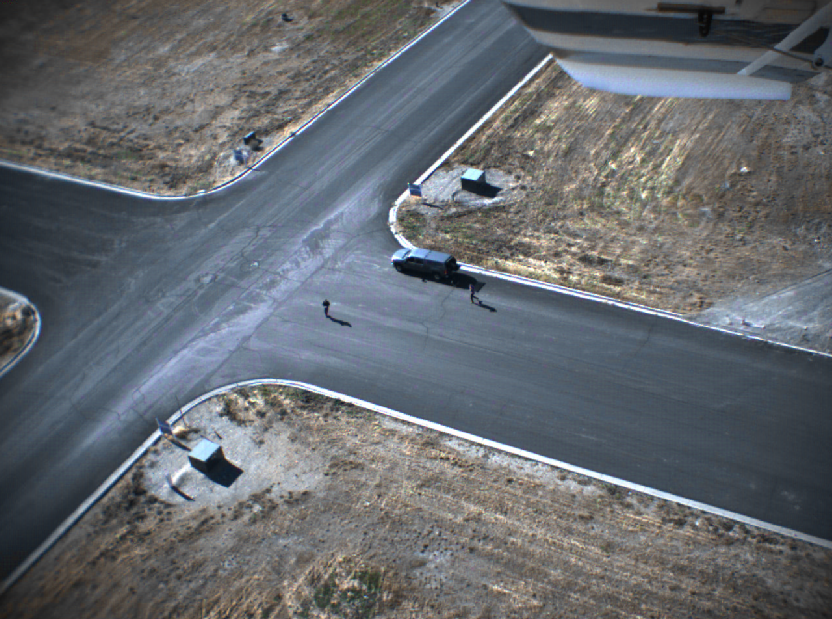
\includegraphics[width=.45\textwidth]{gimbal_far.png}
		\caption{\textit{This image shows the observed targets from a low-cost small UAV. As can be seen, the targets are difficult to observe and this makes them difficult to track.}} 
		\label{fig:gimbal_far}
	\end{center}
\end{figure}


\begin{figure*}
	\begin{center}
		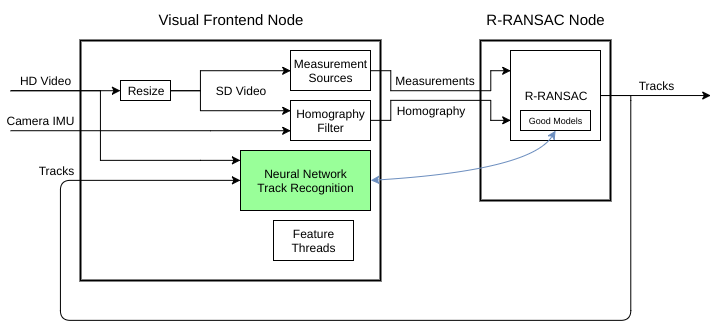
\includegraphics[width=.85\textwidth]{rransac.png}
		\caption{\textit{This block diagram shows how a neural network plays a roll in the Visual MTT framework. The scope of the work for this project is shown in green.}} 
		\label{fig:rransac}
	\end{center}
\end{figure*}

%%%%%%%%%%%%%%%%%%%%%%%%%%%%%%%%%%%%%%%%%%%%%%%%%%%%%%%%%%%%%%%%%%%%%%%%%%%%%%%%
\section{BACKGROUND AND MOTIVATION} \label{BACKGROUND}

\begin{figure}
	\begin{center}
		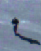
\includegraphics[width=.45\textwidth]{gimbal_zoomed.png}
		\caption{\textit{This image shows the observed targets that has been digitally zoomed in on.}} 
		\label{fig:gimbal_zoomed}
	\end{center}
\end{figure}


In most use cases of military UAV's, ISR missions are primarily used to track ground targets that are of interest to the military. Receiving reliable intelligence about the ground target can be critical in saving the lives of many. Accurate information about what they are tracking and who they are tracking is extremely important because receiving wrong information can result in the undesirable consequence of the loss of innocent lives. Although current military UAV's are very capable in tracking ground targets, unfortunately, there are also many mistakes made and targets are lost. 

\begin{figure*}
	\begin{center}
		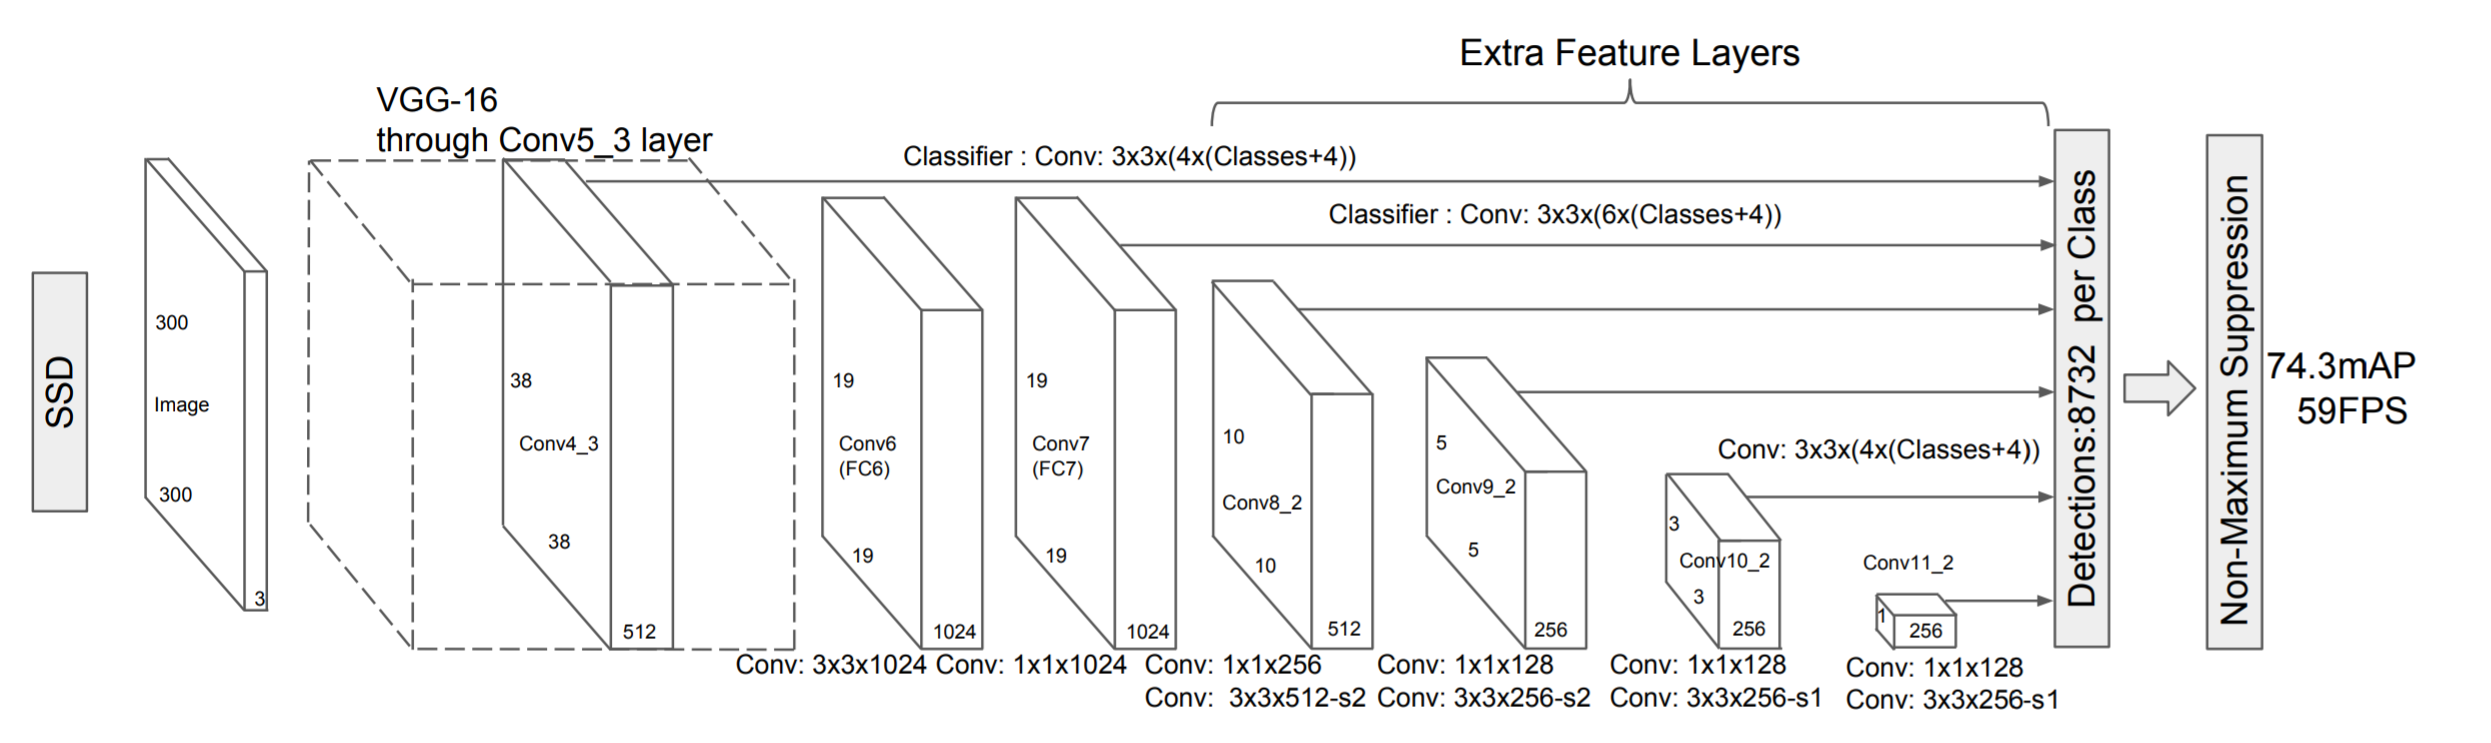
\includegraphics[width=.95\textwidth]{ssd.png}
		\caption{\textit{The SSD network from \cite{liu2016ssd}. It is a modified version of the VGG-16 network.}} 
		\label{fig:ssd}
	\end{center}
\end{figure*}

Lost ground targets are the result of a couple of factors. The first factor is that when viewing a target from a high altitude and a far distance, the target can be blurred by distortions in the air or the target might be low resolution because the capabilities of the camera on-board the aircraft. An example of what a small UAV might observe from a lower-quality camera can be seen in Figure \ref{fig:gimbal_far}. To make matters worse, the resolution quickly degrades as the image is digitally zoomed on the target as can be seen in Figure \ref{fig:gimbal_zoomed}. This same problem exists for larger, more expensive military grade UAV's, but to a lesser degree. Often, however, the larger UAV's are observing the target from much farther away and at a higher altitude.

The second factor in why targets are lost is because of human error. The military currently uses pilots/co-pilots to visually track the target on the ground using a video feed they receive back at their ground station. This video feed is subject to temporary glitches in the streaming service that can cause interruption of the video. Upon regaining the video feed, the gimbaled camera may need to be realigned with the target. Given the image as observed in Figure \ref{fig:gimbal_far}, this may be difficult for a human operator to do if the scene is in a cluttered, pattern-like environment such as a city. The operator may not be able to visually recognize the desired target anymore. Human operators are also subject to boredom and fatigue when tracking a ground target for many hours. 


Work has been done to make target tracking autonomous and relatively robust. In \cite{niedfeldt2014multiple}, a method of tracking multiple targets using an algorithm called recursive random sample consensus (R-RANSAC) was developed at Brigham Young University for tracking multiple moving ground targets. This paper discusses the difficulties of tracking ground targets using computer vision methods because of noisy and spurious measurements, missed detections, and the interaction between multiple maneuvering targets. The method in \cite{niedfeldt2014multiple} presents a way to track moving targets by estimating their dynamic states using a Kalman filter. This is able to be done because of a linear acceleration model. R-RANSAC assumes that the target won't suddenly teleport or instantaneously stop or change directions. With this assumption, the Kalman filter can estimate and track the target by estimating the next state using the dynamics of a linear acceleration model. This method provides a great way to robustly track a continuously observed target that is constantly moving while being very computationally lightweight and efficient.

R-RANSAC, however, is subject to some limitations. One of the primary limitations of R-RANSAC is that when a target is temporarily unobserved, i.e. the target goes off the frame of the camera or the target moves behind an occlusion, the target is lost. The other main limitation with R-RANSAC is its inability to track static targets. If a target were to stop momentarily and then continue on, R-RANSAC would initialize a new track and make no correlation between the new track and the old one. It is the same case for when a target is temporarily blocked from the field of view.

Work has also been done to improve R-RANSAC in \cite{ingersoll2015vision} and its data association problem. A Sequence Model (SM), which is a machine learner, is presented in \cite{ingersoll2015vision} to improve the data association from target tracks created by R-RANSAC. This is done by learning where the target location is in an inertial reference frame. This work greatly improved the ability for R-RANSAC to associate targets with previous target tracks by remembering where the target was last seen. However, error in measurements again still cause for lot of error to enter the system and often targets that were observed multiple times are often not associated with previous target tracks. Therefore, R-RANSAC still classifies them as new targets. 

There has also been numerous papers published about how neural networks could be used in target tracking. There are online decision making algorithms as presented in \cite{xiang2015learning} that uses Markov decision process to model the lifetime of an object. This method deserves further investigation with application to the problem discussed in this paper. However, it is unclear how computationally heavy this algorithm is. 

Other papers such as \cite{sadeghian2017tracking}, \cite{choi2015near}, and \cite{keuper2016multi} all present different methods on how do deal with tracking multiple targets. The methods presented in these papers, however, are all computationally too heavy for a small embedded computer on a small UAV.

When only one object is observed, reinforcement learning can be a great approach such as in \cite{zhang2017deep}, \cite{choi2017visual}, \cite{yoo2017action}, and \cite{luo2017end}. These papers present much more computationally efficient ways to track a target; however, in the case of our problem where multiple targets are present, these solutions will not work.

The most promising solutions for our problem are presented in \cite{liu2016ssd} and \cite{redmon2016you}. In \cite{liu2016ssd}, the single shot multibox detector (SSD) presents a very computationally efficient way of tracking multiple targets. The SSD network uses the VGG-16 as a base and convert two of the fully connected layers to convolutional layers, subsample parameters from those fully connected layers, and use the \textit{a trous} algorithm \cite{holschneider1990real} to fill in the gaps. The SSD network illustration from \cite{liu2016ssd} is shown in figure \ref{fig:ssd}. This network was chosen to be a base example for our problem because of its streamlined computational efficiency which even beat out YOLO from \cite{redmon2016you} as far as performance speed.

\begin{figure}
	\begin{center}
		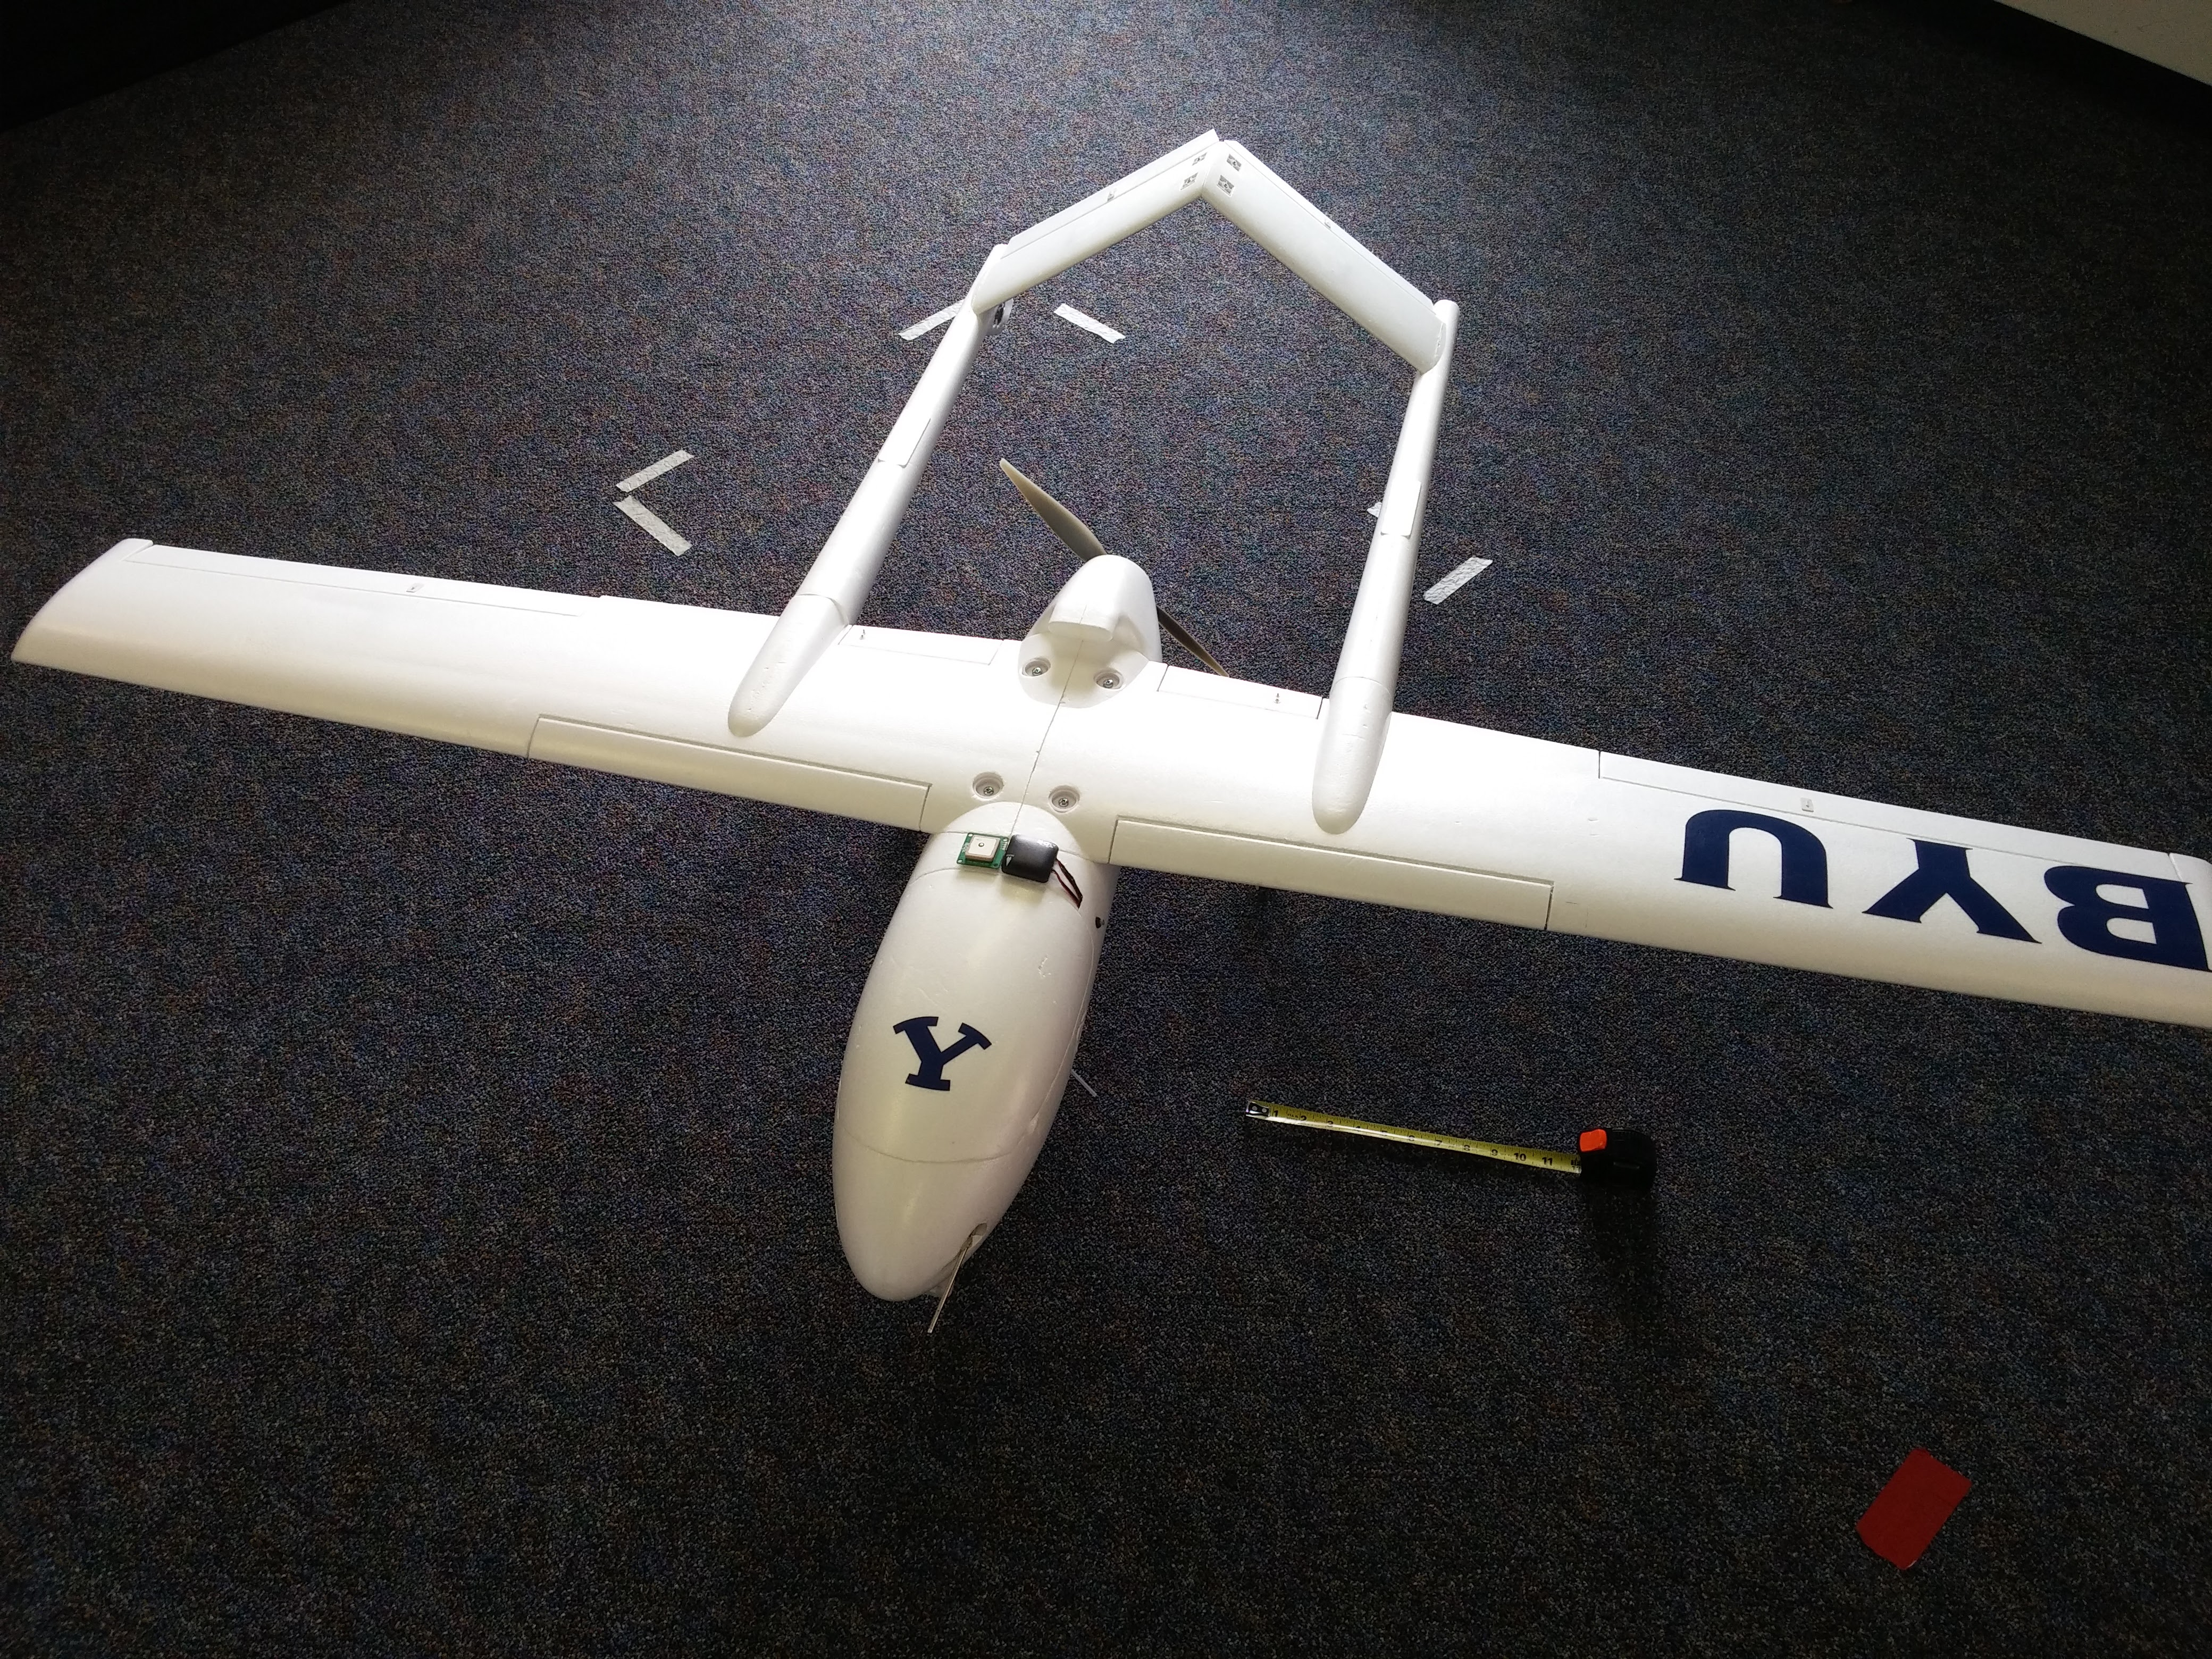
\includegraphics[width=.45\textwidth]{anaconda.jpg}
		\caption{\textit{This is the Anaconda UAV. This aircraft is what we used to collect our data for this project. Its wingspan is 7 feet.}} 
		\label{fig:anaconda}
	\end{center}
\end{figure}


\section{DATA ANALYSIS} \label{DATA}

\subsection{Data Collection}
Most of the time spent for this project went towards collecting good data that we could use to train and test our network. Unfortunately, this process took way longer than expected. First, a set of data was collected from a small fixed-wing UAV so the results would be as real as possible. 

To simplify things, only two targets were present during the collection of the video data. This was intentionally the case to make the training and testing of the neural network much faster and simpler. We used the Anaconda UAV from Ready Made RC products. This aircraft is capable of flying for an hour while carrying on-board a gimbaled camera and an embedded computer. This aircraft can be seen in Figure \ref{fig:anaconda}. The camera we used was a low-cost global shutter camera called the Point Gray Chameleon. It was on a two-axis gimbal mechanism that allowed the camera to pan and tilt. This camera setup can be seen in Figure \ref{fig:gimbal}. The images shown in \ref{fig:gimbal_far} and \ref{fig:gimbal_zoomed} are from this UAV and camera setup. The video was recorded on-board so we could test our neural network through several iterations.

\begin{figure}
	\begin{center}
		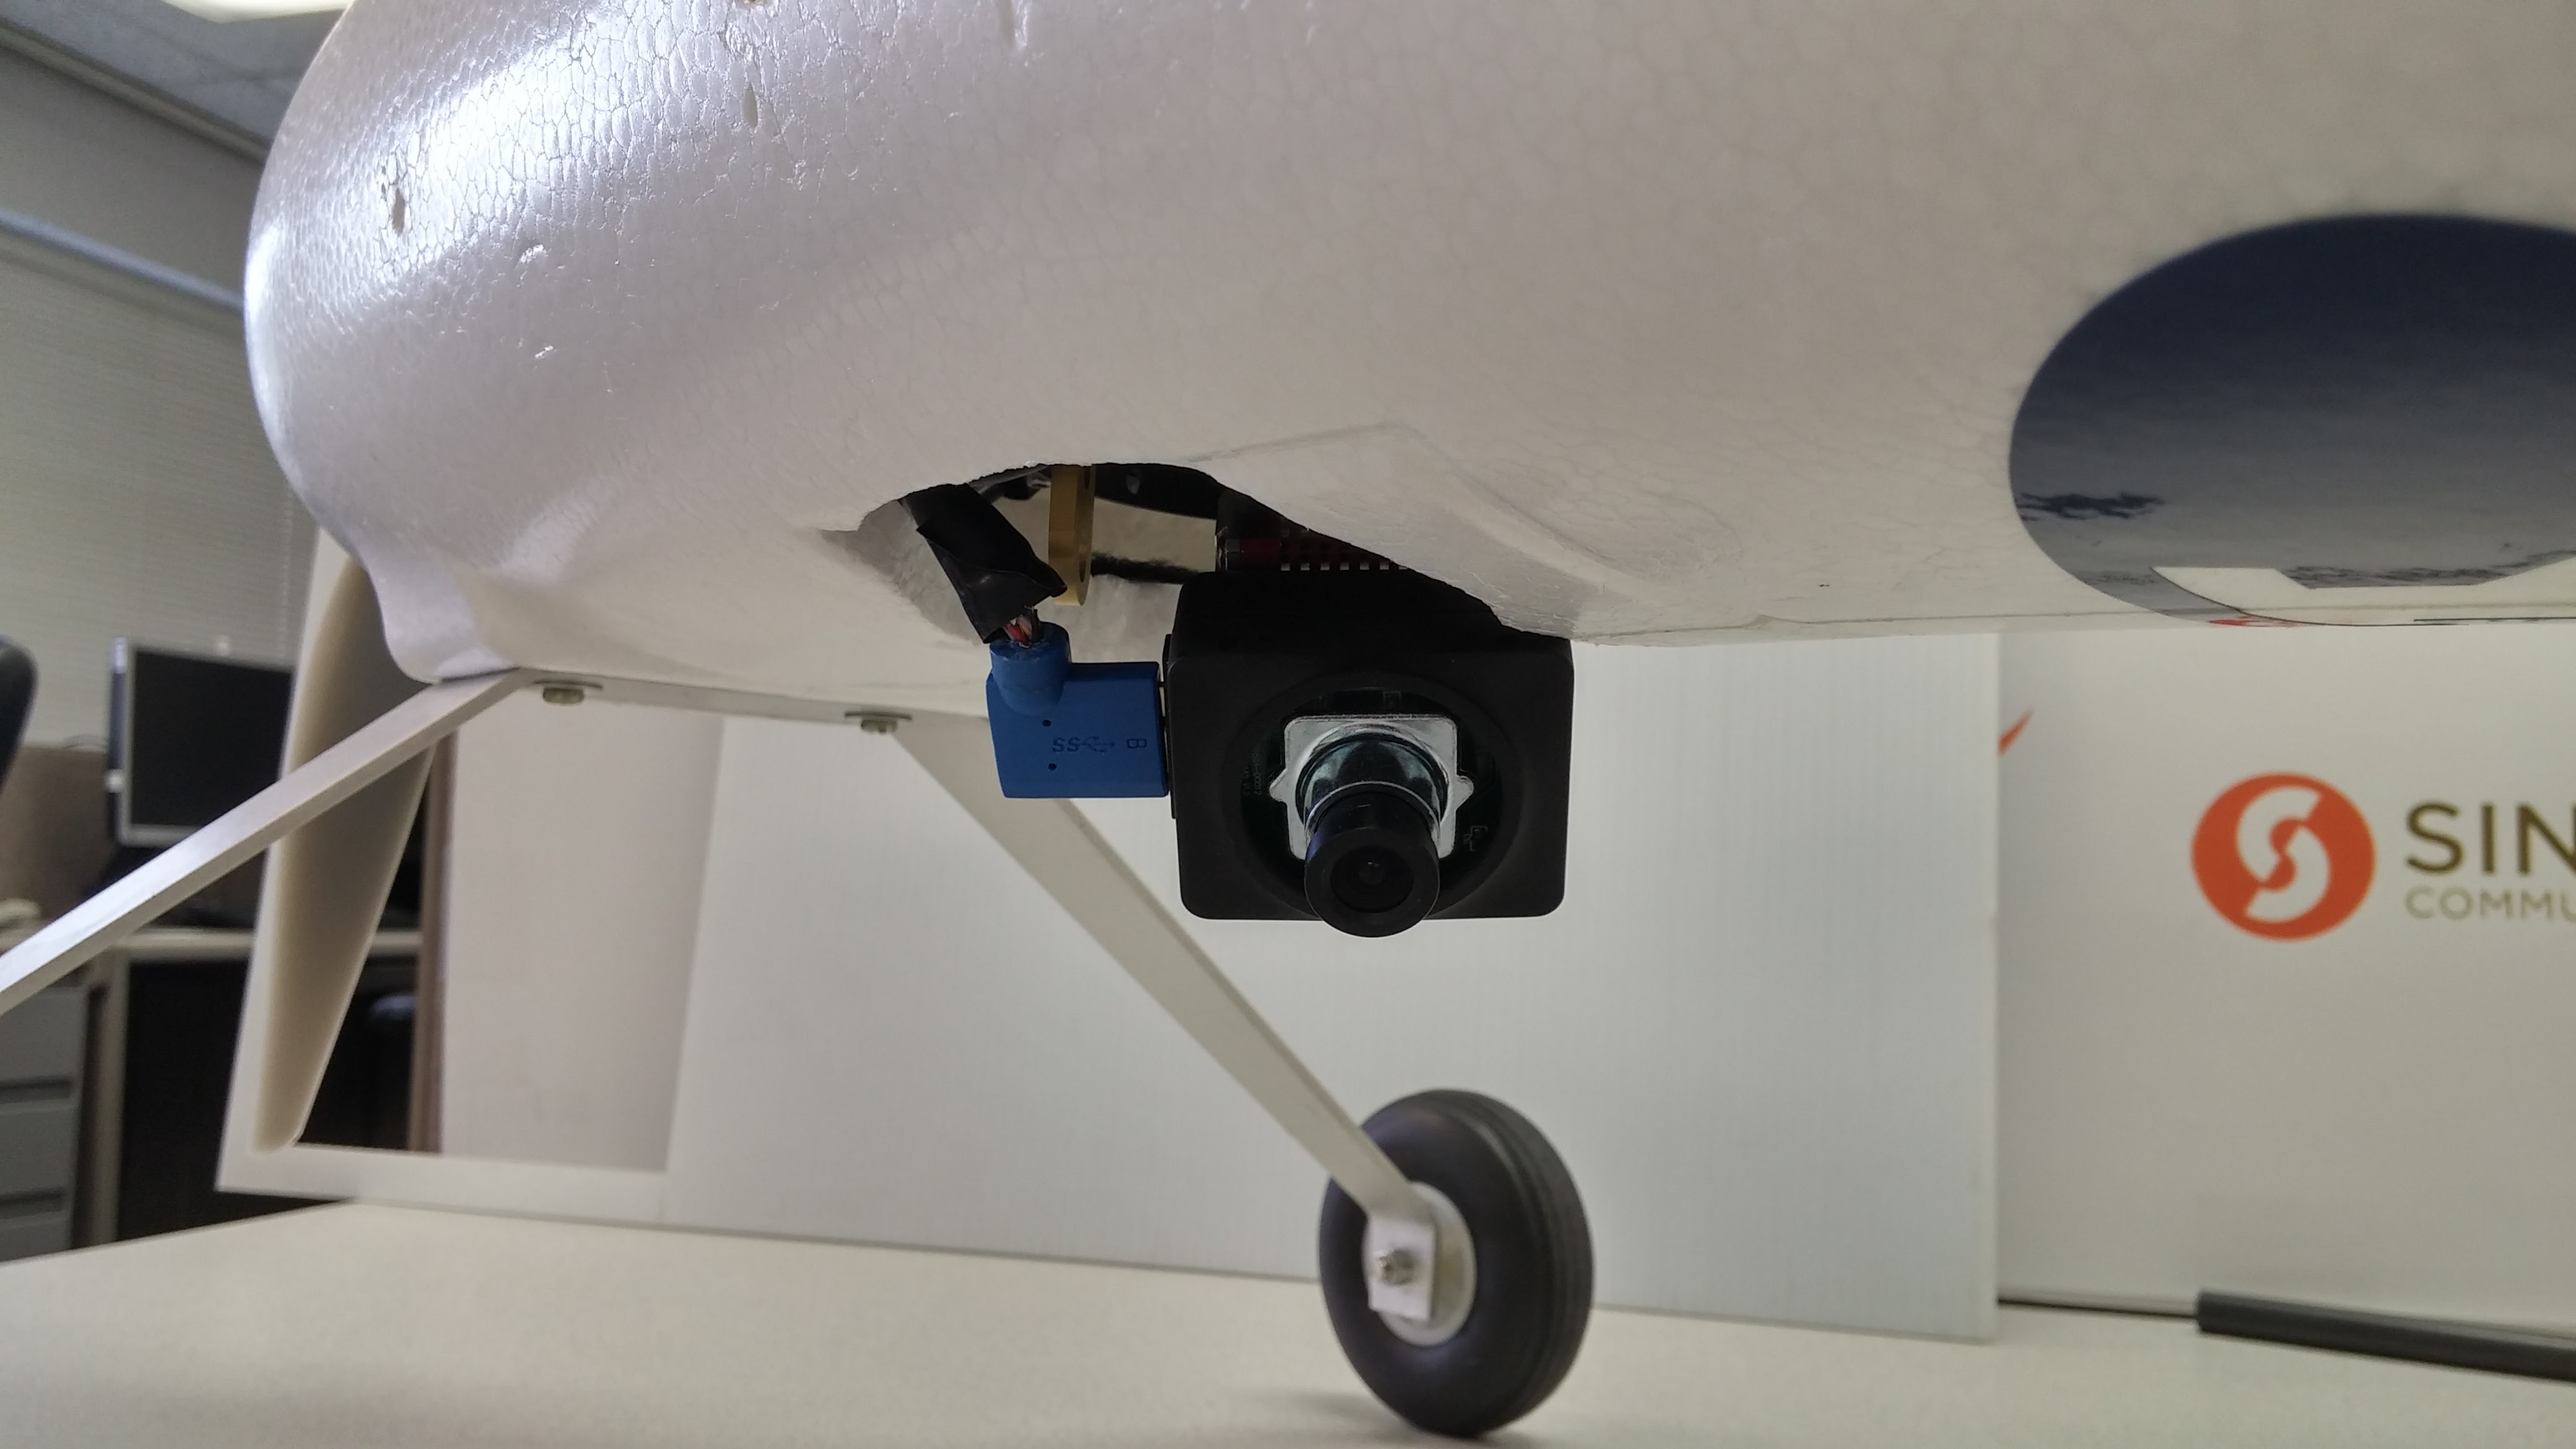
\includegraphics[width=.45\textwidth]{gimbal.jpg}
		\caption{\textit{This Point Grey Chameleon camera attached to a gimbal is what was used to collect the video data.}} 
		\label{fig:gimbal}
	\end{center}
\end{figure}

\subsection{DATA PRE-PROCESSING}

After collecting the data, we needed a way to process the video data so that we could crop the image around the target and feed it to our neural network. This task, however, proved to be difficult. Originally, the plan was to use the work developed in our research group here at Brigham Young University in tracking the targets in the video. More work has been done to \cite{ingersoll2015vision} and \cite{niedfeldt2014multiple} to improve the tracking capabilities. The frame work in these papers has been modified and put into the Robot Operating System (ROS) framework. This new framework for tracking targets using R-RANSAC is called Visual Multi-Target Tracking (Visual MTT). The Visual MTT architecture is new research and has yet to be published in another paper. That publication is forthcoming.

In attempting to use the Visual MTT algorithm to observe the moving targets, although it was fairly reliable in observing moving objects, it wasn't very reliable at predicting the center mass of the object in the image. This meant that when attempting to use the reference point given from the output of the Visual MTT framework as the center point where we should crop our image around to give to the neural network to train/classify, the cropped image often gave a result of the image from behind or in front of the target. This was difficult to debug and caused a lot of problems in trying to train our network since the network would train on images that were not the target most of the time. 

Another issue with using the data collected from the Anaconda UAV was that the cropped view of the targets had so little resolution that unless the target were wearing completely different colors, any difference between the targets was unobservable. This can be seen in Figure \ref{fig:gimbal_2}. This figure shows the second target that can be seen in \ref{fig:gimbal_far}. Therefore, this data was not going to work.

\begin{figure}
	\begin{center}
		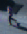
\includegraphics[width=.45\textwidth]{gimbal_zoomed_2.png}
		\caption{\textit{This image shows a second target that has been digitally zoomed in on.}} 
		\label{fig:gimbal_2}
	\end{center}
\end{figure}

In order to progress faster with the development of the neural network, a video was recorded from on-top of the Joseph F. Smith Building at BYU. This video was recorded for another project prior to this project. The camera was set on a tripod and the video was still. This allowed for simple background subtraction to annotate the targets in the video. A resulting image from the annotated video can be seen in Figure \ref{fig:jfsb}. This provided much clearer targets as can be seen in Figure \ref{fig:jfsb_zoomed}. Even these images, however, were still not good enough for training a neural network. Although large color differences could be observed, several of the people were wearing similar colors. This made it nearly impossible for the network to distinguish one target from another. Another issue with this data set was that almost no targets would be obstructed at any time and then return to the line of sight. The dataset that was used in this project is discussed in section \ref{METHODS}. 

\begin{figure}
	\begin{center}
		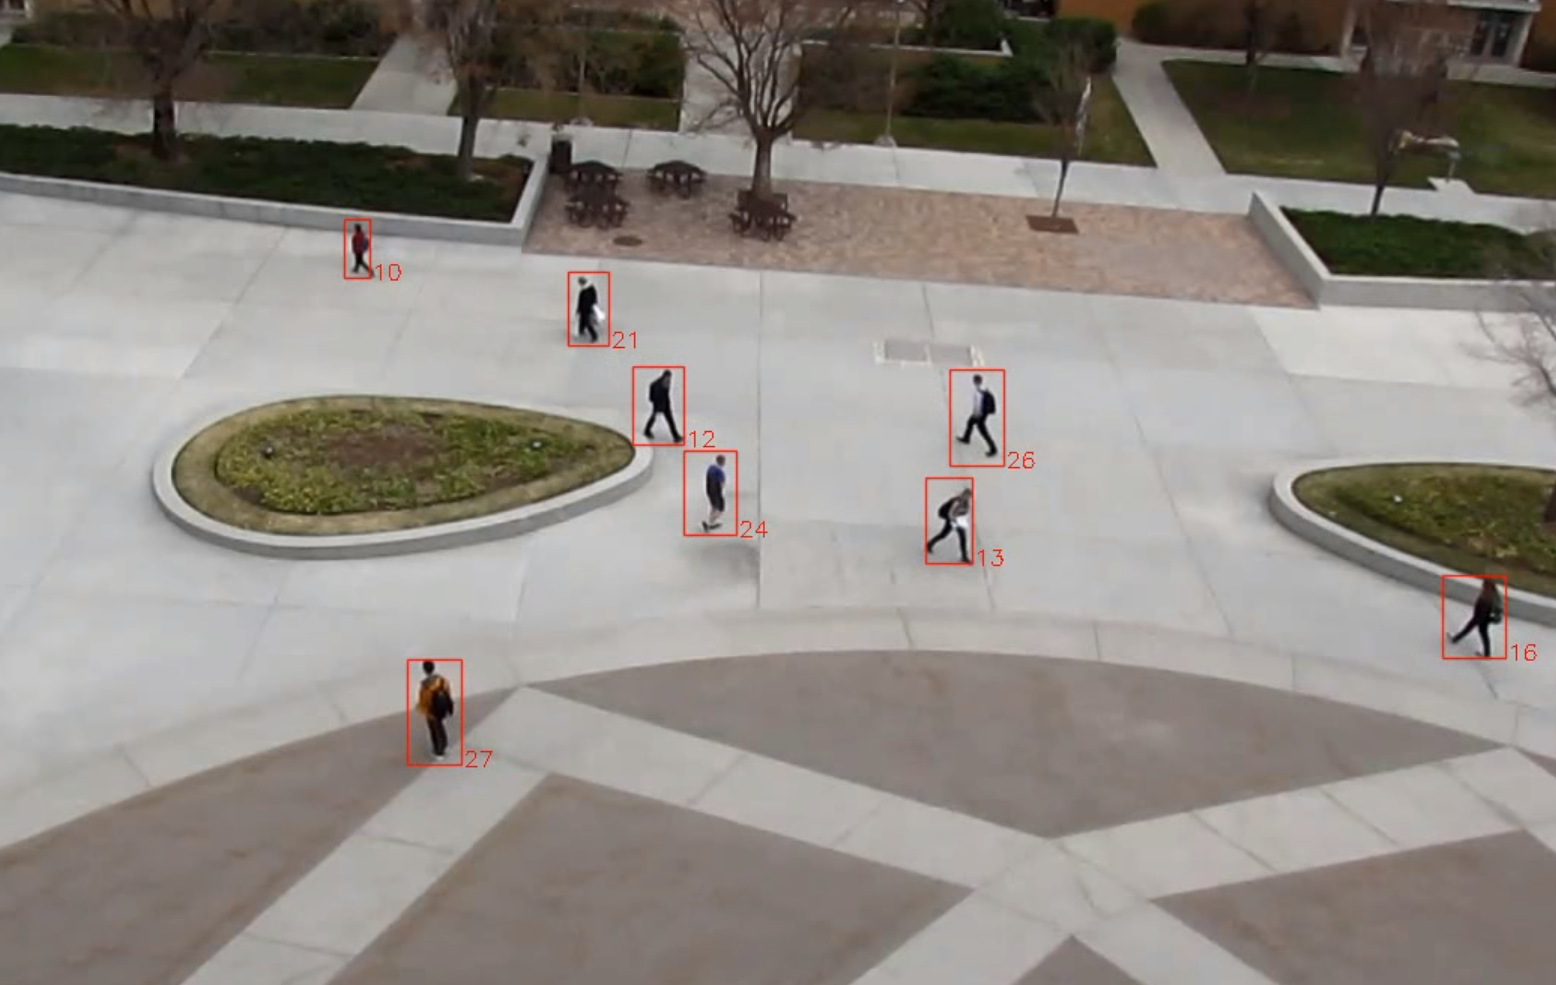
\includegraphics[width=.45\textwidth]{jfsb.png}
		\caption{\textit{This is a still image from video recorded from a stationary camera on top of a building.}} 
		\label{fig:jfsb}
	\end{center}
\end{figure}

\begin{figure}
	\begin{center}
		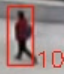
\includegraphics[width=.45\textwidth]{jfsb_zoomed.png}
		\caption{\textit{This is a still image from video recorded from a stationary camera on top of a building.}} 
		\label{fig:jfsb_zoomed}
	\end{center}
\end{figure}

%%%%%%%%%%%%%%%%%%%%%%%%%%%%%%%%%%%%%%%%%%%%%%%%%%%%%%%%%%%%%%%%%%%%%%%%%%%%%%%%%%
\section{METHODS} \label{METHODS}

In this section we will discuss the technical approach to creating a neural network to classify and identify targets. Much of the work so far in the project consisted of acquiring good data and preprocessing that data to provide reliable consistent images for the neural network to train on. Eventually the goal is to connect this neural network to the Visual MTT framework as shown in Figure \ref{fig:rransac}. In developing the neural network, however, the annotations provided in the dataset will be used in place of the Visual MTT framework.

\subsection{Quantitative Metric}

One of the benefits to using the Atrium dataset provided by \cite{jodoin2014urban} is that all targets visible in the video are annotated throughout the whole video. Each target, however, is assigned a new target identification each time the target disappears from the field of view and the reappears in the image frame. This allows us to easily test the neural network after training as if it is receiving a new track ID from Visual MTT. To measure the accuracy, however, that had to be tracked by hand. This wasn't too difficult because there were only 7 individual people shown in the video. That meant that after the network saw the first 7 unique people, the rest of the track identifiers were repeats. This was measured by hand by pausing the program periodically and viewing the image in the video and the output of the neural network. A more scientific method could be derived if more time were permitted.

\subsection{Data Preparation} 

Ultimately, a dataset was found that has been made publicly available from \cite{jodoin2014urban}. We used the Atrium dataset from this paper. This dataset came with clear images of pedestrians walking around with different colored clothes. The background color, as can be seen in Figure \ref{fig:atrium_full} is also very different from the color of the pedestrian. This dataset also came with background subtracted images along with detailed annotations. These annotations and background subtracted images is what would be used in training and testing the neural network. It is worth noting that one of the time consuming parts of using this dataset was that the annotations and background subtracted images were indexed differently than the actual video image. This issue caused a massive delay in setting up the network. Using the annotations provided by the data set, each target image was cropped down a $60\times170$ pixel image from the center point of the annotation. This size was chosen because it was the median size for all of the annotations. Any target image that didn't meet this minimum size was not used in the training or testing of the neural network. The image size had to be of fixed width and height to easily pass into the VGG-16 network. The final result of the cropping can be seen in Figure \ref{fig:atrium_combined}.

\begin{figure}
	\begin{center}
		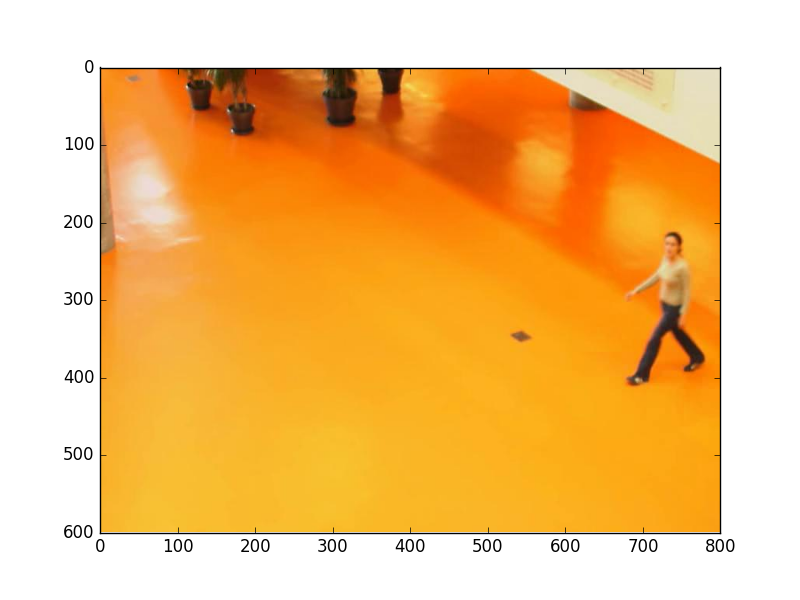
\includegraphics[width=.45\textwidth]{atrium_full.png}
		\caption{\textit{A still image from the Atrium dataset from \cite{jodoin2014urban}.}} 
		\label{fig:atrium_full}
	\end{center}
\end{figure}

\begin{figure}
	\begin{center}
		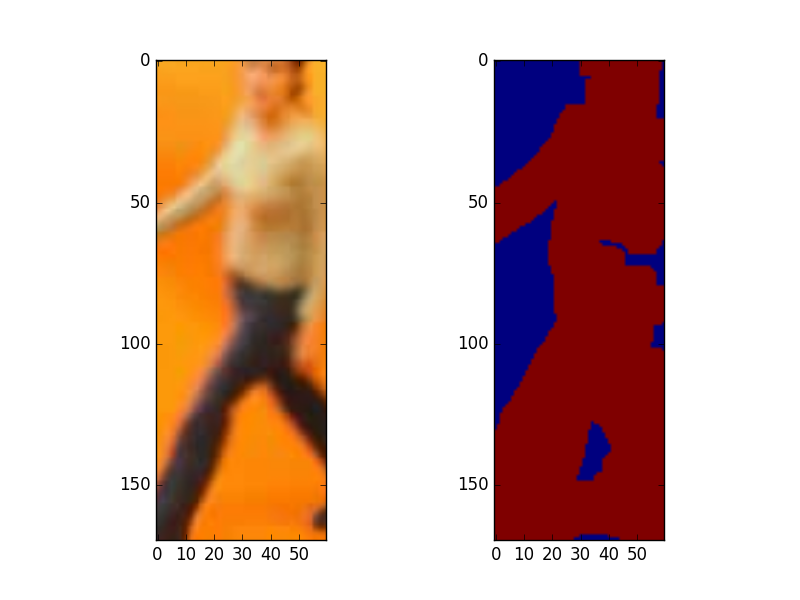
\includegraphics[width=.45\textwidth]{atrium_combined.png}
		\caption{\textit{Cropped target image and matching background subtracted image. These images were used in the training of the network.}} 
		\label{fig:atrium_combined}
	\end{center}
\end{figure}

One trick that was use to improve results was that for each camera frame that came in, we made a copy of the horizontally flipped image. This allowed for the network to always train on at least two images at a time and not just over fit to each image as it comes in. 

\begin{figure*}
	\begin{center}
		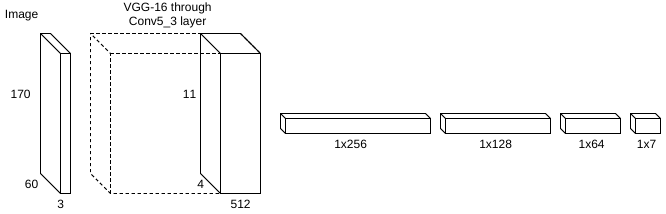
\includegraphics[width=.95\textwidth]{cnn.png}
		\caption{\textit{This was the final network used in this project.}} 
		\label{fig:cnn}
	\end{center}
\end{figure*}

\subsection{Neural Network}

The neural network that ended up being used in this report was a convolutional neural network (CNN) since the primary purpose of the network was a classification problem. In an attempt to make it robust and speedy, the first attempt at constructing a neural network was in following the SSD architecture given in \cite{liu2016ssd}. This architecture promised good results; however, we were unable to get this network to work. This was certainly a bug in the code. However, many hours were spent in trying to solve this problem and the problem persisted. 

The network that was ultimately used was the VGG-16 network through convolution 5-3. Then four fully connected layers were constructed with output sizes of 256, 128, 64, and 7, in that order. An illustration of this network can be seen in Figure \ref{fig:cnn}. This was a fairly traditional CNN. The primary way this CNN was unique was in the way data was passed to the CNN. With only one frame coming in at a time from a live video feed, this means that the network can only train on a few images at a time. When multiple targets were in the camera image, the network would be able to train on more than just one target. This caused several issues with feeding the network because the batch size was now a variable size. For this reason, I was unable to get the network to train. The loss function was the sparse softmax cross entropy between the label and the fourth fully connected layer.

\section{RESULTS AND DISCUSSION} \label{RESULTS}

Unfortunately, I was unable to get the network to train and classify the images. This is primarily because of the way a live video feed comes into the network. With traditional classification problems, training the network typically allows for passing in several images at a time in a batch. With a video streaming in, one target is viewed at a time. This can be problematic when training because the network can easily over fit for that one target. The other issue is that the network seems to need a variety of different classes to train against so that when it comes time to classify a target, it has multiple models to choose from. I have yet to come up with a way that tells the network when to train and when to start classifying. 

Although I was unable to get the network to train successfully, a lot was learned in the process of collecting and processing the image data. Ultimately, the goal of this project was to run a lightweight network that was computationally efficient enough to be implemented on our UAV's flight computer, an NVIDIA Jetson TX2, as shown in Figure \ref{fig:tx2}. Part of the reason why the images were so far cropped down was to improve the speed at which the network would run. Attempting to crop the image to a small size that just barely fit the target without some kind of truth, such as the annotations found in the Atrium dataset, proved to be a really difficult task. Relying on motion detection and the Visual MTT framework to provide a good center point for the target caused much hardship in trying to train a network. I learned that the Visual MTT framework may not be entirely suitable for the approach of cropping the image around the target and then sending that through a neural net to train on. A better approach for a neural network track recognition component for the MTT framework would be to implement something such as the SSD network on the full image. The computational resources of the TX2 flight computer could still be moderately conserved if the network only ran when Visual MTT picked up a new track. Further investigation into this will be done outside of the scope of this project.

A significant amount of time was given in reviewing the literature for this project and it was found that the SSD network seemed most promising for multiple targets. It seemed that CNN's were the most common when it came to classifying multiple targets. Another approach to this problem, however, would be to use a recurrent neural network (RNN) for each single target that is tracked by the Visual MTT framework. RNN's are very good at tracking objects in motion and it could prove to be valuable when the targets are highly occluded. Perhaps even a joint CNN and RNN for detecting and tracking the target could be used as proposed in \cite{fangtrack}.

\begin{figure}
	\begin{center}
		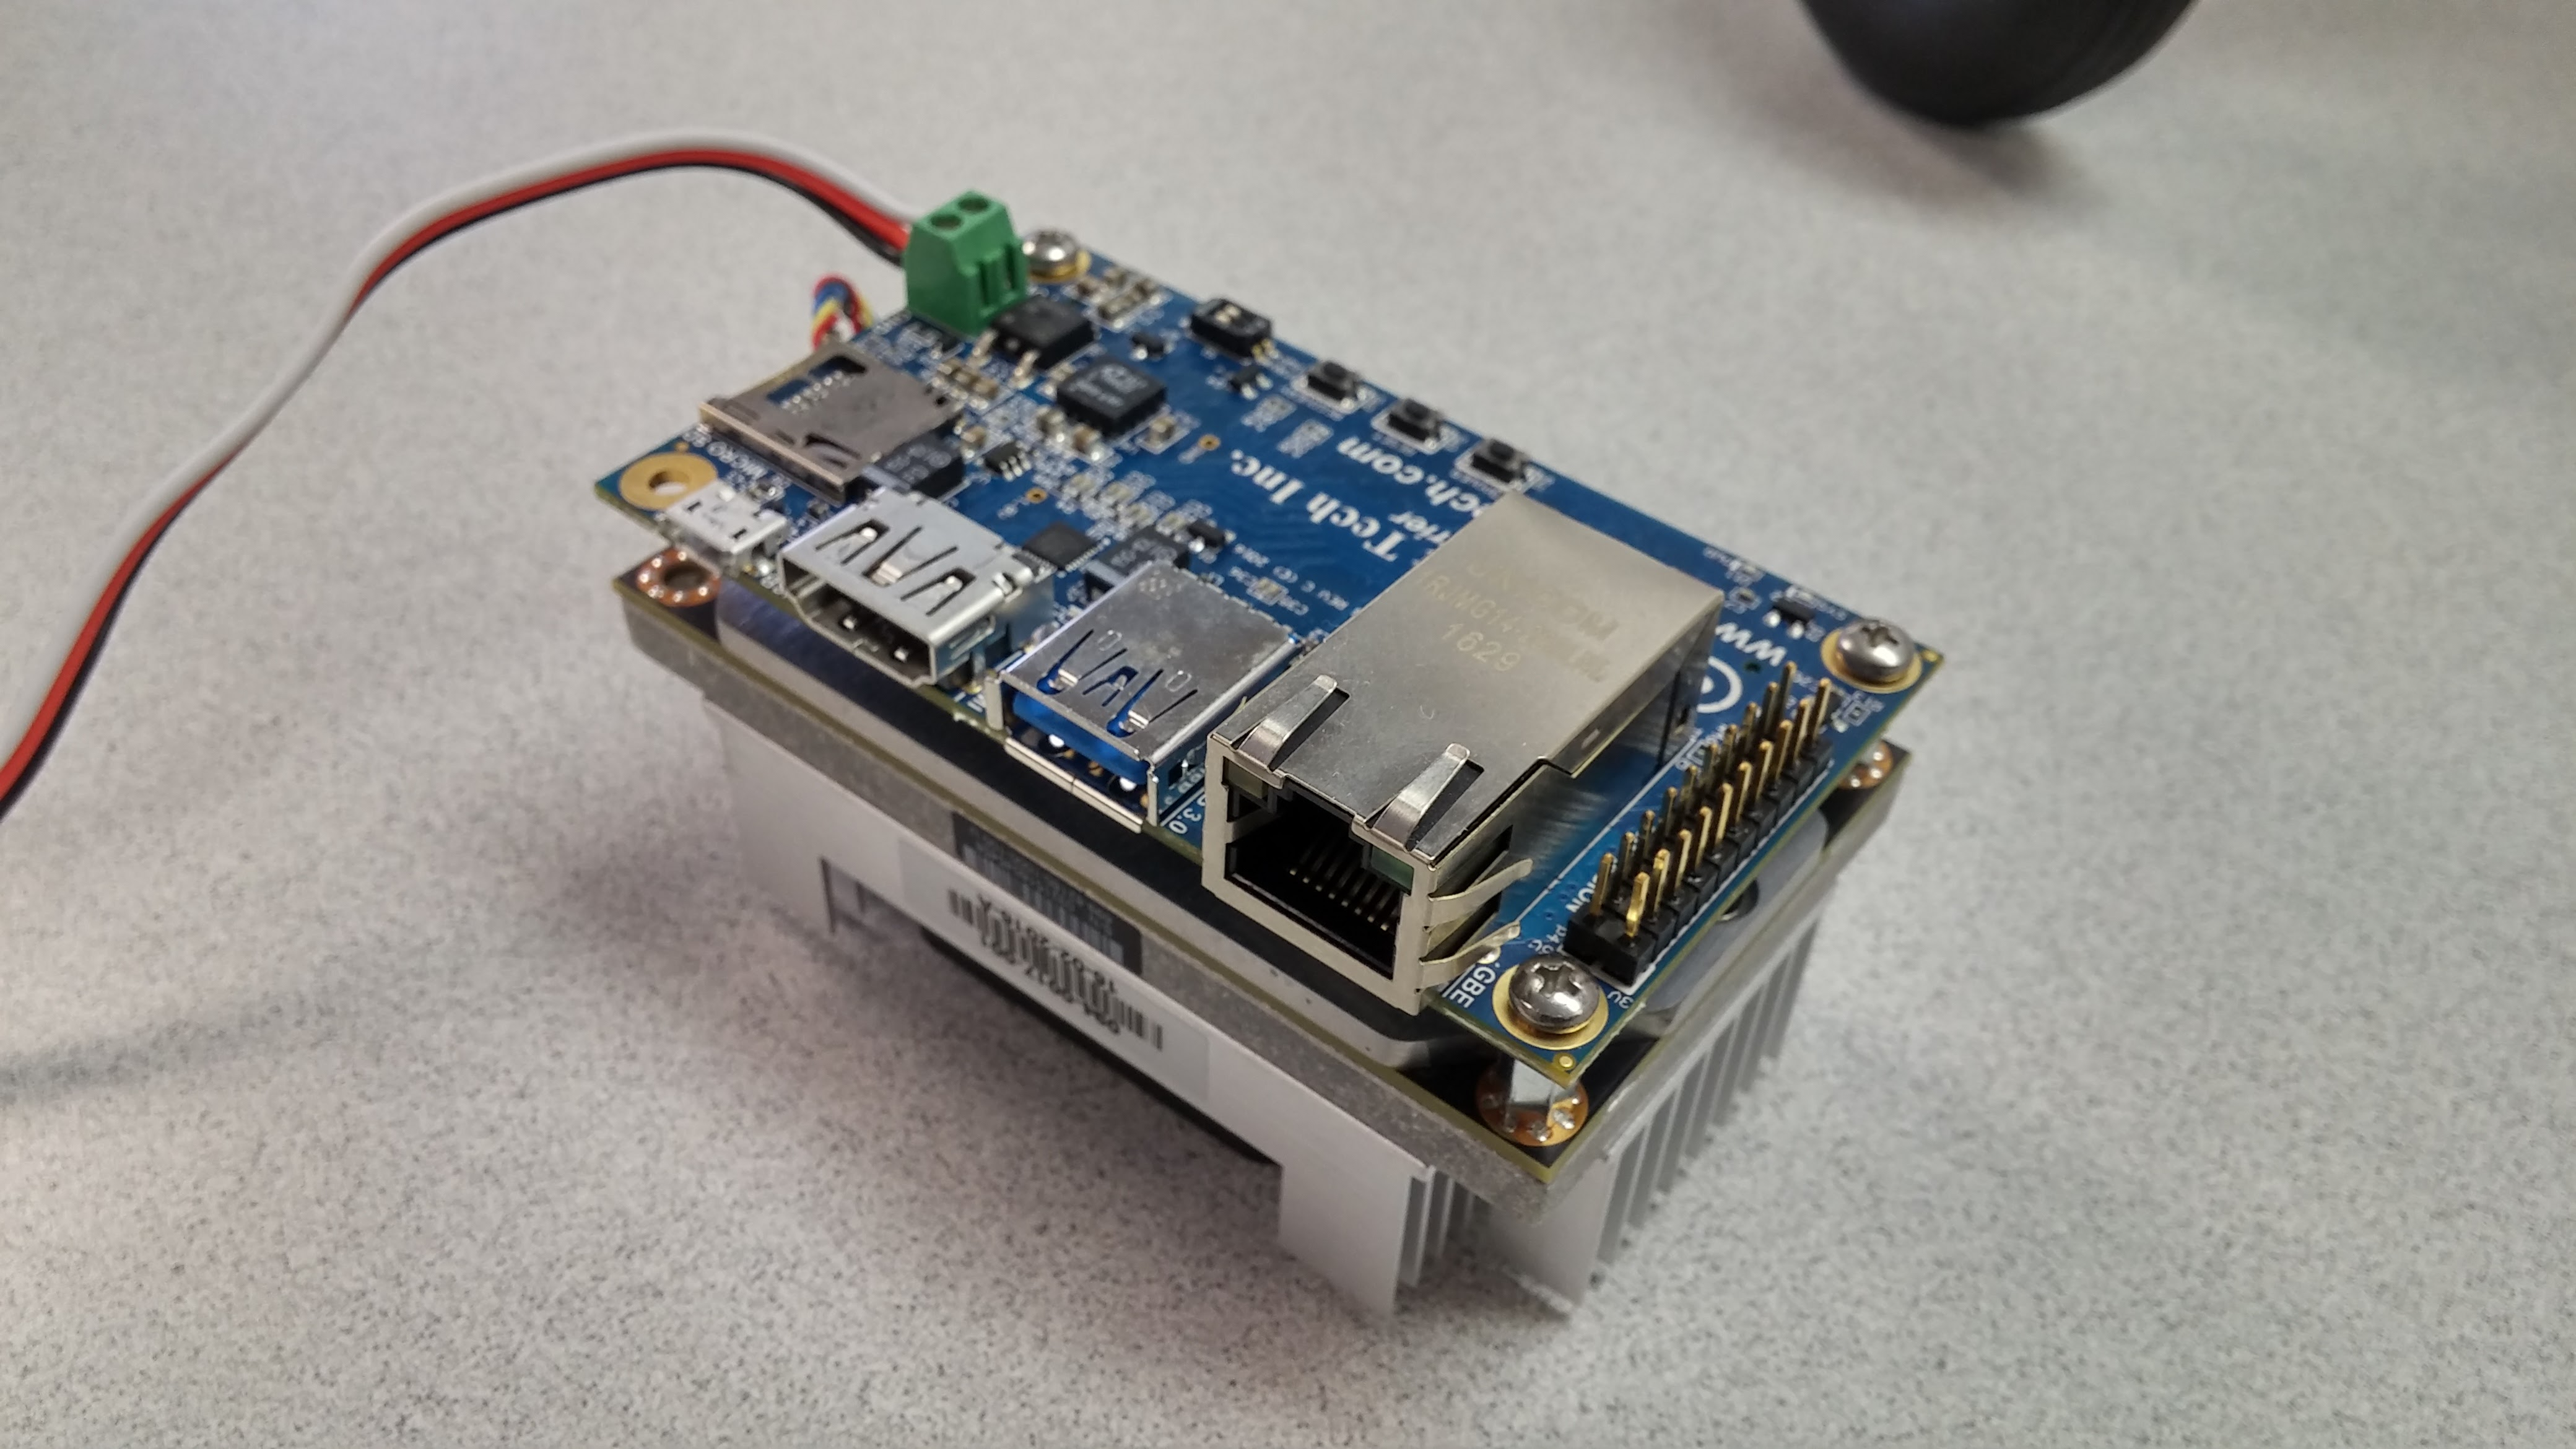
\includegraphics[width=.45\textwidth]{tx2.jpg}
		\caption{\textit{The NVIDIA Jetson TX2 computer is used as an on-board flight computer. It has a low-power GPU that is capable of running lightweight neural networks.}} 
		\label{fig:tx2}
	\end{center}
\end{figure}

%%%%%%%%%%%%%%%%%%%%%%%%%%%%%%%%%%%%%%%%%%%%%%%%%%%%%%%%%%%%%%%%%%%%%%%%%%%%%%%%%%

\section{CONCLUSION} \label{CONCLUSION}

This project was a difficult project. In total, I recorded at least 45 hours in researching, debugging, and writing. I spent the first 12 hours reading and researching different papers on how neural networks apply towards target tracking. Most of what I read about were neural networks that were very successful at tracking targets robustly, but were also very computationally heavy. Many of the algorithms presented in the references given were only able to run at a few frames per second on very expensive, heavy, and powerful graphics cards. While this works great for some ground based system, it is not feasible for small UAV's.

The SSD network appears to be one of the fastest networks that is designed for tracking objects. For this reason, a modified version of it was selected to attempt to make a classification network for the Visual MTT process. Further debugging is required to get the network training on streaming video images coming into the network. 

A significant amount of time was also spent in collecting and processing data for the project. In total, approximately 23 hours were spent in this section of the project. The reason so much time was given to collecting the data was because we did not have any video data of multiple moving targets on the ground from a fixed-wing UAV. The video data that was collected for the purpose of this project will be useful for research in the BYU MAGICC lab in the future. After the first video data was found to be unusable for this project, the next dataset that was attempted was the video recorded from the top of the JFSB. Using background subtraction to extract a pseudo truth bounding box around moving targets also proved difficult for this project as the camera's auto-focus was often trying to refocus the camera. As a result, many of the bounding boxes around the targets had a lot of error and again it caused issues with training a neural network. Finally, the Atrium dataset was found and this was very useful. Indexing to the correct image with the correct bounding box for each target, however, also proved to be a very difficult task because of how the dataset was labeled. Learning how to deal with no targets in an image, to one or many targets in an image was also a useful experience. A lot of time was given to solving indexing issues here.

The remainder 10 hours given to the project went into writing this report. Part of why so much effort was given to this report was in the hopes that in a few weeks when I get this network running with Visual MTT, we can actually submit a conference paper since this would be a unique contribution, especially to the community that is trying to track targets autonomously with small UAV's. 

Although the end result of the neural network is currently disappointing, I learned a lot in the process. One of the core concepts I learned was to start with the most simplified data you can possibly start with. Several hours would have been save had I found the Atrium dataset at the beginning of the project. I also learned a lot about the current capabilities of neural networks in detecting and classifying objects. This has been valuable research for my thesis work as I am attempting to track multiple targets from a small UAV. The research done for this project will be continued on over the next several weeks to possibly make a more robust target tracker. 

%%%%%%%%%%%%%%%%%%%%%%%%%%%%%%%%%%%%%%%%%%%%%%%%%%%%%%%%%%%%%%%%%%%%%%%%%%%%%%%%
% \section*{APPENDIX}

% Appendixes should appear before the acknowledgment.

% \section*{ACKNOWLEDGMENT}

% Important people/organizations who made it possible


%%%%%%%%%%%%%%%%%%%%%%%%%%%%%%%%%%%%%%%%%%%%%%%%%%%%%%%%%%%%%%%%%%%%%%%%%%%%%%%%

\bibliography{./library}
\bibliographystyle{ieeetr}



\end{document}


%%%%%%%%%%%%%%%%%%%%%%%%%%%%%%%%%%%%%%%%%%%%%%%%%%%%%%%%%%%%%%%%%%%%%%%%%%%%%

% SAVED STUFF






%new document




